\chapter{Background}
\label{chapter:background} 

First in this section brief details of JVM are examined.
Second, general concepts of software quality and SQA are explained.
Third, SQA practice automated testing is inspected in more detail.
After this, agile methodologies Test Driven Development \textbf{(TDD)}, Acceptance Test Driven Development
\textbf{(ATDD)} and Behavior Driven Development \textbf{(BDD)} are reviewed. For the last section in this chapter,
related research on the thesis study topic is presented.

\section{Java Virtual Machine} %1p
    JVM and its programming language Java was originally designed for building software on networked devices~\cite{lindholm2015java}. From there
    next major usage possibilities for Java came from Web HTML-sites. Web-sites with Java embedded programs first appeared in HotJava-browser~\cite{lindholm2015java}.
    From those days usage of Java has explored new fields and JVM itself hosts nowadays many more programming languages than
    just Java~\cite{wiki:jvm}.

    JVM is an \textbf{abstract computing machine} that provides instruction set and different memory areas at runtime.
    Current implementations of JVM have brought the environment to mobile, desktop and server devices, yet the JVM itself
    isn't tied to any specific technology. The basic information for JVM comes from \textit{class} files. These files include
    binary JVM bytecode instructions. Instead of having Java code in class files, it compiles to these binary instructions
    that are run on JVM. Figure \ref{fig:JVM} illustrates the runtime memory areas and the class loader system.
    JVM has support for \textit{primitive} and \textit{reference} types, from which latter enables support for referencing JVM objects. ~\cite{lindholm2015java}

    JVM is interesting target for a vast amount of programming languages, thanks to its maturity, ubiquity and performance~\cite{sarimbekov2013characteristics}.
    These programming languages pass as a valid JVM language if their functionality can be expressed in a valid class file~\cite{wiki:jvm}.
    Programs written in ported dynamic languages such as \textit{Ruby (JRuby)} or \textit{Python (Jython)}~\cite{sarimbekov2013characteristics} can be run on the JVM.
    JVM also hosts an array of new programming languages such as \textit{Scala, Clojure} and \textit{Groovy}~\cite{wiki:jvm}.

    The possibilities of these additional JVM programming languages are crucial part of this thesis. Later on testing Java-code is examined with
    different implementation level BDD-testing frameworks from various JVM languages.

    \begin{figure}[ht]
      \begin{center}
        \includegraphics[width=12cm]{images/jvm.png}
        \caption{Overview of internal architecture of Java Virtual Machine}
        \label{fig:JVM}
      \end{center}
    \end{figure}

\section{Software quality assurance}
    The standard definition of quality assurance states it to be:
        \textit{"A planned and systematic pattern
        of all actions necessary to provide adequate confidence
        that the item or product conforms to established
        technical requirements"}.~\cite{buckley1978standard}
    Although modern software quality assurance differs from the original standard definition, it is still definitely found
    at the core of SQA. To fully understand SQA and why it is important, first the software quality concept in itself is illustrated.
    Motivation for practicing SQA is examined second and third the overall activities in SQA are explained briefly.
    \subsection{Definitions of quality}
    Quality in software development is a multifaceted entity that has had many viewpoints for a long time.
    Some of these earlier views include \textit{product, transcendental, user, manufacturing} and \textit{value based} view~\cite{kitchenham1996elusive}.
    Because there exists so many viewpoints to what software quality is, it makes the measuring of quality hard~\cite{kitchenham1996elusive}.
    Business goals and their priorities should determine the needed level of software quality~\cite{kitchenham1996elusive} so therefore
    quality in itself is not set in stone, but it can alter between software services and products to fit the purpose.
    This can be easily demonstrated with an example of software inside a missile defence system or an online dating application.
    Two different systems with different goals and consequences of use and therefore obviously different standards for needed quality.

    \begin{figure}[ht]
      \begin{center}
        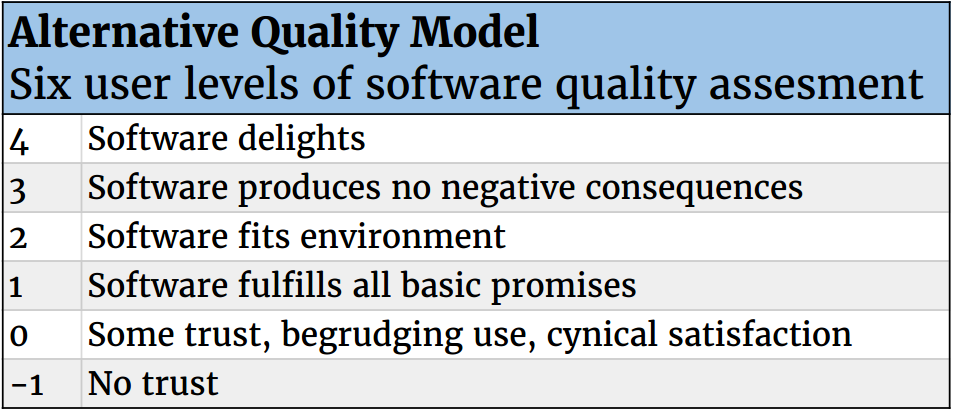
\includegraphics[width=10cm]{images/alternativeQM.png}
        \caption{Alternative Quality Model}
        \label{fig:AQM}
      \end{center}
    \end{figure}

    New alternative view on software quality by Denning~\cite{denning2016sq} includes user experience directly in the core of quality.
    This view is called the \textbf{alternative quality model (AQM)} and it defines quality software as software that delights
    the end user~\cite{denning2016sq}. Figure \ref{fig:AQM} displays the full scale of AQM.
    While this research is mainly interested in aspects of producing traditional defect free quality software,
    later on in this chapter BDD is examined in detail. BDD can be seen to directly try to increase software quality on the AQM,
    providing value for end users and other stakeholders while at the same time minimizing defects~\cite{chelimsky2010rspec}.

    \subsection{Motivation for SQA}
    Many software projects fail but also many of them are successful. Success and failure in this context have multidimensional meaning with
    \textit{technical, economic, behavioral, psychological} and \textit{political} aspects ~\cite{mcleod2011factors}. Aggressive
    schedule can be usually seen as one of the primary causes for software project failure~\cite{cerpa2009did}. This can cause
    problems on many of the projects multidimensional axis, for instance in technical- and economical aspects. Projects might go
    over the budget, schedule, not meet the user needs and eventually be released with low quality ~\cite{cerpa2009did}.
    Although many of the problems are related to requirements engineering \textbf{(RE)}, a lot of them are fixes or rework needed after launch~\cite{lessons}.
    If quality is measured on the AQM, then both RE and SQA are intertwined in the concept of software quality and SQA-work
    is essential for the success of software project. Even if software quality is only limited to mean defect free software, SQA has
    major role in preventing project failures.

    \subsection{Activities in SQA}
    Quality assurance practices and activities differ greatly in rhythm and also to a lesser degree in practices used in
    traditional waterfall-model software projects vs agile projects~\cite{huo2004software}. Waterfall-projects have a rule set
    of their own for quality assurance, but for the topic of thesis agile methodologies and their SQA-practices are more relevant.
    SQA-practices can be generally categorized to \textit{defect detection, code enhancement, verification \& validation (V\&V)} of artifacts,
    and \textit{collaboration \& communication} between stakeholders.

    Defect detection can be split into two categories: \textbf{explicit} and \textbf{implicit} defect detection activities~\cite{mantyla2014software}.
    Implicit defect detection means finding defects as a secondary result when the goal was to perform another activity,
    such as demo presentation or giving training about the software use~\cite{mantyla2014software}. Explicit defect detection activities
    hold ones such as \textit{testing} and artifact \textit{inspection}, but they are found to have a lower
    defect detection rate than implicit ones~\cite{mantyla2014software}. \textit{Continuous integration} can also be seen
    as a explicit defect detection as it illustrates integration defects and problems with frequent integration cycle~\cite{huo2004software}.

    Code enhancement activities aim to produce better design and maintainability of the codebase and these include practices
    like \textit{pair programming, refactoring}~\cite{huo2004software} and \textit{code reviews}~\cite{rigby2013convergent}.
    Although code reviews are also a form of inspection and explicit defect detection, one of their primary uses in modern
    code review is to share knowledge between team members~\cite{mantyla2014software}~\cite{rigby2013convergent}.

    Verification \& Validation aims to guarantee the quality of product or intermediate products and it can be used for
    example to design and requirement artifacts. It is a static method, which involves stakeholder(s)
    inspecting the artifact. It is more of a traditional waterfall software project activity, but agile practices such as code reviews
    can be categorized as a V\&V activity. ~\cite{huo2004software}

    Collaboration and communication between stakeholders are used in agile methodologies frequently being one of the
    cornerstones of agile practices in general~\cite{huo2004software}. Frequent customer collaboration with \textit{On-site customer}~\cite{huo2004software}
    is an agile SQA-practice that establishes a foundation for many agile practices and is essential in delivering
    quality on the AQM.

    There are many more specific SQA practices that have their foundations on the activities mentioned in this section.
    Next in this thesis testing is examined in detail through automated testing as it provides a base for agile SQA practices \textbf{TDD},
    \textbf{ATDD} and \textbf{BDD}.

\section{Automated testing}
    First in this section different levels of test automation are explored. Second lower levels of test automation are explained in more
    detail and third overall benefits and drawbacks of test automation are discussed.

    \subsection{Levels of automation}
    \begin{figure}[ht]
      \begin{center}
        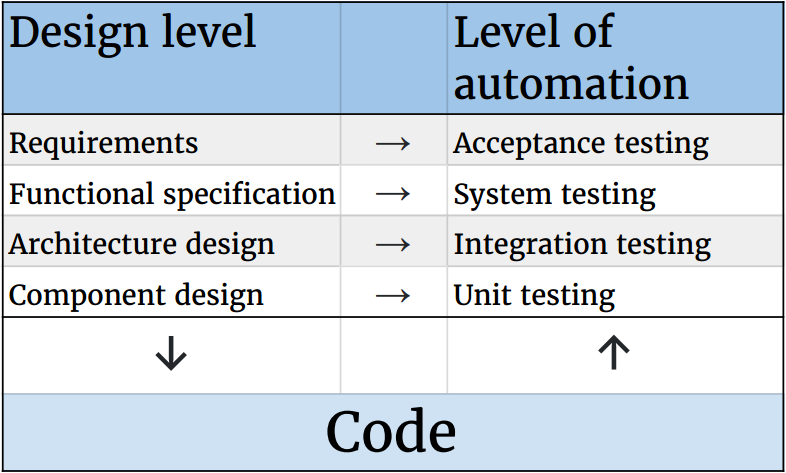
\includegraphics[width=10cm]{images/testlevels.png}
        \caption{Test last development regarding system and its design}
        \label{fig:testlevels}
      \end{center}
    \end{figure}

    Test automation comes at many levels of granularity regarding the system and its requirements. The four main levels for
    functional testing are \textit{unit, integration, system} and \textit{acceptance} testing~\cite{itkonen2016}.
    Figure \ref{fig:testlevels} illustrates how different levels of design relate to levels of test automation in traditional
    \textbf{Test Last Development (TLD)}. At the bottom
    of figure \ref{fig:testlevels} there is code, which is the result of design and foundation (in traditional automated testing)
    for different testing levels. Different levels of design guide the automated tests at the specified level.

    The introduced test automation levels are a part of functional testing. There exists also different non-functional
    requirements for software projects that can be automatically tested, such as \textit{performance} and \textit{security} testing~\cite{crispin2009agile}.
    These are not in the scope of this study, instead the functional testing levels of automated unit and integration testing are
    the main topic of interest.

    \subsection{Low level testing explained}
    Low level testing in the scope of this thesis means automated unit and integration level testing. They both have separate
    definitions and usages inside software projects, but the distinction between the two can be found confusing by many developers~\cite{artofunit2013}.
    Figure \ref{fig:testlevels} illustrates how unit testing adheres to component design and integration testing to architecture design ~\cite{itkonen2016}.

    \textbf{Unit test} has many similar definitions which all agree that it tests individual unit or collection of these units working as one
    ~\cite{runeson2006survey}~\cite{whittaker2000software}. Unit test also has the property of being isolated from the rest
    of the system~\cite{whittaker2000software}. Unit testing can in a sense also be seen as an intersection of design,
    coding and debugging~\cite{langr2015pragmatic}.
    Dedicated practitioner of unit testing Osherove~\cite{artofunit2013} has identified important aspects of a good unit test:
    \textit{trustworthiness, maintainability, readability, isolated,} has \textit{single concern} and contains \textit{minimal repetition}.

    \textbf{Isolation} is an important part of unit testing. This means in practice using test doubles also known as \textit{mocks}.
    Using mocks in unit tests means substituting real objects with limited functionality provided by mocks. Mocks can be
    configured to behave always in a specified manner. This configured behavior of mocks is called \textit{stubbing},
    in which output result of mock object can be injected from the test code. Traditional uses of mocks are for instance using
    them to make progress without implementing dependencies (used in TDD/BDD), isolating unit under test from dependencies
    or nondeterminism. ~\cite{chelimsky2010rspec}

    \textbf{Integration testing} is the second, higher level of automated testing in the low level testing scope of thesis.
    The definitions of integration testing state that it is a testing
    activity which involves multiple components~\cite{whittaker2000software}~\cite{artofunit2013}. Osherove~\cite{artofunit2013}
    defines integration testing as testing a unit of work with real dependencies in place, for instance database and  networking.
    Integration tests are not usually as fasts as unit tests~\cite{artofunit2013}. Many times this results from including
    full context of the system through dependency injection container, such as \textit{Spring Framework} or \textit{Guice}~\cite{kapelonis2016java}.

    \subsection{Benefits and drawbacks}

    \begin{table}[H]
        \begin{center}
            \begin{tabular}{ | p{6.3cm} | p{6.3cm} |}
            \hline
            \textbf{Benefits} & \textbf{Drawbacks} \\ \hline
            Rapid feedback~\cite{prechelt2016quality} & Can't replace manual testing~\cite{rafi2012benefits} \\ \hline
            Improved product quality~\cite{rafi2012benefits}~\cite{williams2009effectiveness} & Maintaining difficulty~\cite{rafi2012benefits}~\cite{runeson2006survey} \\ \hline
            Increased test coverage~\cite{rafi2012benefits} & Lack of skilled people~\cite{rafi2012benefits}~\cite{runeson2006survey} \\ \hline
            Increased developer confidence~\cite{rafi2012benefits} & Hard to select correct testing strategies~\cite{rafi2012benefits}~\cite{berner2005observations} \\ \hline
            Reduced testing time~\cite{rafi2012benefits} & Brittle tests~\cite{berner2005observations} \\ \hline
            Shorter release cycle~\cite{berner2005observations} & More development time~\cite{williams2009effectiveness} \\ \hline
            Increased testability design~\cite{berner2005observations} & Cost versus value~\cite{runeson2006survey} \\ \hline
            Act as documentation~\cite{langr2015pragmatic}~\cite{chelimsky2010rspec}~\cite{kapelonis2016java} & Unmaintaned tests can lose all value~\cite{berner2005observations} \\ \hline
            Continuous regression~\cite{williams2009effectiveness} &  \\ \hline
            \end{tabular}
            \caption {Automated Testing Benefits \& Drawbacks} \label{tab:automated-title}
        \end{center}
    \end{table}
    Agile methodologies do not prefer or deny separate testers inside a project, but for a modern quality centered
    development separate testers might hinder the experience~\cite{prechelt2016quality}. Teams without separate testers have one aspect in common,
    they rely heavily on test automation as the core of quality. One of the most important properties in these kind of
    teams is the rapid and direct feedback that test automation can provide~\cite{prechelt2016quality}. Overall the task of test automation
    doesn't come with benefits only, but it has also its drawbacks.

    \textbf{Benefits} of test automation are vast. Systematic literature review by Rafi et al.~\cite{rafi2012benefits} has found many
    of them through various sources. Some of them can be highlighted: \textit{improved product quality, test coverage increase,
    increase in developer confidence} and \textit{reduced testing time}.

    Automated testing was found also to allow \textit{shorter release cycles}. This is a result of
    tests executed more often and therefore allowing defects to be detected earlier with reduced cost to fix.
    Quality and depth of test cases also increase with automation, as less time is needed for executing them and more time is available
    to design the test cases. Another benefit of automated testing is the more layered, testable design of the software.
    To achieve the \textbf{benefits}, test automation \textbf{strategy needs to combine different approaches} and testing levels. ~\cite{berner2005observations}

    Automated test cases can also \textbf{help to understand} the system. This is enabled by writing information how the production code should behave
    into the test cases and test methods. ~\cite{langr2015pragmatic}~\cite{chelimsky2010rspec}~\cite{kapelonis2016java}

    At unit testing level, benefits of test automation was found to include over 20\% decrease in test defects~\cite{williams2009effectiveness}.
    Also the defects found by largely increased customer base in first 2 years of use was decreased by introducing unit testing practices~\cite{williams2009effectiveness}.
    Another strength of automated unit testing is also the continuous regression suite it provides~\cite{runeson2006survey}.

    Unfortunately test automation isn't only beneficial compared to manual testing. In the earlier mentioned review by Rafi et al.~\cite{rafi2012benefits}
    some of the \textbf{limitations} include for instance: \textit{automation can't replace manual testing, difficulty in maintaining}
    and \textit{lack of skilled people} for test automation. Usually the lack of skilled people tends to result in projects as
    \textit{inapporiate test automation strategies}~\cite{rafi2012benefits}~\cite{berner2005observations}. These kind of projects
    usually automate testing at wrong levels, for instance automatically testing through Graphical User Interface (GUI). This
    can lead to brittle tests that are hard to maintain as the GUI changes~\cite{berner2005observations}. Neglecting automated
    testing maintenance can lead to knowledge diminishing and tests that lose totally their capability to run~\cite{berner2005observations}.
    Altogether testware maintenance is hard and this can be many times seen as tests that are not engineered
    with the same attention to detail as actual production code~\cite{berner2005observations}.

    At unit testing level, drawbacks of test automation include approximately 30\% more development time compared to manual testing~\cite{williams2009effectiveness}.
    Runeson~\cite{runeson2006survey} also found unit testing drawbacks similar to the afore mentioned automated testing problems by other studies.
    These include \textit{unit testing of GUI}, \textit{competency of developers} working with unit tests and \textit{unit test maintenance}~\cite{runeson2006survey} .
    Also the cost of unit test versus the value it provides was found problematic amongst unit testing practitioners~\cite{runeson2006survey}.

    The next sections agile methodologies TDD, ATDD and BDD are all build on top of automated testing practices, operating on different levels
    of automation.

\section{Test Driven Development} %2p
    \subsection{Definition}
    Kent Beck~\cite{beck2003test} defines TDD as techniques aimed to produce clean code that works.
    This is done by driving development with automated tests - Test Driven Development. TDD consists of two basic rules:
    \textit{write new production code only when automated test fails} and
    \textit{eliminate duplicated code}. These two rules are the base for \textbf{Red-Green cycle} of TDD:

    \begin{enumerate}
    \item \textbf{Red}: Design and write a small simple test. Run it and see it fail.
    \item \textbf{Green}: Add code sufficient to make the earlier written test pass.
    \item \textbf{Refactor}: Refactor for clean code. Improve the structure of the production code and test code.
    Run all tests to ensure refactoring didn't break anything.
    \item \textbf{Repeat}: Repeat the cycle to add more functionality.
    \end{enumerate}
    \begin{figure}[ht]
      \begin{center}
        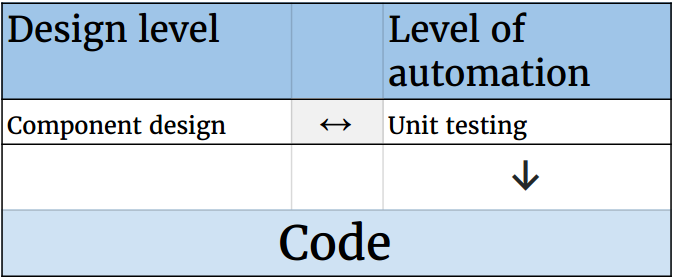
\includegraphics[width=10.0cm]{images/tdd.png}
        \caption{TDD related to system design}
        \label{fig:TDD}
      \end{center}
    \end{figure}
    The tests written in TDD cycle are unit tests, providing incremental functionality to small pieces of software at a time~\cite{bissi2016effects}.
    Beck~\cite{beck2001aim} also defines test-first principle to be much more than just testing and he states that TDD is
    also a software design technique. Figure \ref{fig:TDD} illustrates how component design and unit testing are now in a relation
    where both can affect each other. Code is produced only through design captured in unit tests.

    \subsection{Benefits and drawbacks}

    \begin{table}[H]
        \begin{center}
            \begin{tabular}{ | p{6.3cm} | p{6.3cm} |}
            \hline
            \textbf{Benefits} & \textbf{Drawbacks} \\ \hline
            Increased external quality~\cite{kollanus2010test}~\cite{bissi2016effects} & Increased\newline development time~\cite{kollanus2010test}~\cite{bissi2016effects}~\cite{williams2009effectiveness}  \\ \hline
            Increased test coverage~\cite{bissi2016effects} &  Requires high discipline~\cite{aniche2010most} \\ \hline
            Tests executed more~\cite{williams2009effectiveness} & Can lead to brittle tests~\cite{chelimsky2010rspec}~\cite{astels2006new}~\cite{amodeo2015learning} \\ \hline
            More precise test cases~\cite{williams2009effectiveness} &  \\ \hline
            \end{tabular}
            \caption {TDD Benefits \& Drawbacks} \label{tab:tdd-title}
        \end{center}
    \end{table}
    \textbf{Benefits} of TDD are not totally clear and exact. On earlier systematic literature review by Kollanus~\cite{kollanus2010test} in 2010 there was found
    weak evidence regarding better \textbf{external software quality} with TDD and even less evidence for better \textbf{internal software quality} with TDD.
    In any case, there was still results pointing to better quality, even though evidence was not uniform.
    External quality was measured with two methods, passing acceptance tests done by researchers and number of defects found before
    reported by the customer. Internal quality had multiple metrics, such as \textit{code coverage, number of test cases, method size, cyclomatic complexity}
    and so on. The metrics was found at times contradicting and consensus of internal quality was left unclear.

    In 2016 systematic literature review of TDD by Bissi et al.~\cite{bissi2016effects} the benefits of TDD was found more uniform and quite
    promising. 88\% of studies showed significant increase in external software quality and 76\% of studies identified
    significant increase in internal software quality. This time external quality was measured only with acceptance tests and compared
    to TLD approach. Internal quality was inspected with the only common metric found in the literature: code coverage. It could
    be argued how good of a metric code coverage is for internal quality, but at least the production code has more instructions
    tested with fast and repeatable automated tests when comparing TDD to TLD.

    Some of the more specific benetifs of TDD was found by Williams et al.~\cite{williams2009effectiveness} to include developers
    creating more tests that are executed more frequently. This seems to correlate with earlier mentioned increased internal
    quality measured by test coverage. TDD was also shown to promote more precise and accurate test cases than TLD~\cite{williams2009effectiveness}.

    \textbf{Drawbacks} of TDD was found unanimously to include increase in development time~\cite{kollanus2010test}~\cite{bissi2016effects}~\cite{williams2009effectiveness}.
    For example in the study done by Williams et al.~\cite{williams2009effectiveness} the increase was ranging from 15\% to 35\%.
    As earlier mentioned, Beck~\cite{beck2001aim} defined TDD to be also a design technique. This aspect could make TDD too demanding practice for junior
    level developers~\cite{hammond2012test}.

    TDD \textbf{requires discipline}, that even senior level developers seem to lack when using it. This is shown for example as
    frequent deviation from the basic rule of starting the process with the \textit{simplest test}. Also the \textit{refactoring}
    of test code is frequently omitted by developers of all experience levels. ~\cite{aniche2010most}

    BDD literature frequently states that TDD can have a tendency to shift viewpoint in testing to verifying system state
    rather than behavior of it. This can lead to brittle tests that are tightly coupled to what the object is, instead of
    what the object does. ~\cite{chelimsky2010rspec}~\cite{astels2006new}~\cite{amodeo2015learning}

    In conclusion, it could be said that TDD \textbf{is not} the \textbf{silver bullet} for software development that solves all the quality problems.
    The two systematic reviews mentioned provide somewhat conflicting results. Nevertheless, it could be argued that in the right
    context benefits of TDD outweigh the drawbacks of it.

\section{Acceptance Test Driven Development}
    ATDD is an agile practice that has many forms and names: \textit{Specification by Example, Agile Acceptance Testing, Story Testing} and
    obviously \textit{Acceptance Test Driven Development}~\cite{gartner2012atdd}. BDD inholds also
    ATDD~\cite{gartner2012atdd}, but as later is discovered, it is actually a superset of it.

    ATDD is an collaboration tool for stakeholders of the project~\cite{gartner2012atdd}~\cite{haugset2012automated}. It means driving the
    development with features specified with executable acceptance level tests~\cite{gartner2012atdd}~\cite{haugset2012automated}.
    ATDD can have many formats, such as \textit{Gherkin, Keyword-driven testing and Tabular formats} ~\cite{gartner2012atdd}.

    Instead of traditional automated testing, ATDD can be seen as a mixture of documentation centric traditional RE and communication focused agile RE~\cite{haugset2012automated}.
    The key is the communication and collaboration between stakeholders~\cite{haugset2012automated}. The executable automated tests are a very useful byproduct.
    Although the name of ATDD holds the word acceptance in it, passing tests doesn't mean that the system works perfectly~\cite{gartner2012atdd}. Instead it is
    only a starting point for more quality assurance work; the system is stable enough to be manually tested further~\cite{acceptance2010}.

    \subsection{Benefits and drawbacks}

    \begin{table}[H]
        \begin{center}
            \begin{tabular}{ | p{6.3cm} | p{6.3cm} |}
            \hline
            \textbf{Benefits} & \textbf{Drawbacks} \\ \hline
            Frequent collaboration~\cite{haugset2012automated} & Demands frequent collaboration~\cite{haugset2012automated}  \\ \hline
            Less ambiquity, noise and over-specification in requirements~\cite{haugset2012automated} & Needs active customer~\cite{haugset2012automated}  \\ \hline
            Faster feedback~\cite{haugset2012automated} & High upfront cost~\cite{haugset2012automated}  \\ \hline
            Increased requirement traceability~\cite{hayes2009towards} & Works bad with constantly changing requirements~\cite{haugset2012automated}  \\ \hline
            Increased trust~\cite{haugset2012automated} & Learning curve~\cite{haugset2012automated} \\ \hline
            Increased test coverage~\cite{haugset2012automated} & Not for all contextes~\cite{haugset2012automated}  \\ \hline
            Faster start for new team members~\cite{haugset2012automated} & Requires high discipline~\cite{haugset2012automated}  \\ \hline
            \end{tabular}
            \caption {ATDD Benefits \& Drawbacks} \label{tab:atdd-title}
        \end{center}
    \end{table}
    One of the major \textbf{benefits} of ATDD is the frequent collaboration \& communication between
    the development team and other stakeholders. This improves the understanding of requirements~\cite{haugset2012automated}
    between all people involved. ATDD can potentially reduce the \textit{ambiquity, noise} and \textit{over-specification}~\cite{haugset2012automated}
    in requirements through the use of shared language. ATDD also promotes faster feedback loop~\cite{haugset2012automated} and traceability from requirements
    to code~\cite{hayes2009towards}.

    Eventually the use of ATDD seems to promote high trust between stakeholders involved, although
    this is an incremental process taking time. ATDD also promotes better coverage for testing
    and reduces overhead for new people starting to work with the project. ~\cite{haugset2012automated}

    \textbf{Drawbacks} of ATDD include usually the needed frequent collaboration of stakeholders in it. Customers
    might not have the time and effort needed for low response times of ATDD. ATDD was also found to have a high
    upfront cost, that should scale better overtime. This is not always the case if the requirements change all the time. ~\cite{haugset2012automated}

    ATDD has learning curve for both the development team and customers, and especially the learning curve for customers
    could be found too high to take the method in to use. ATDD is not for all contextes and doesn't work well for all features.
    ATDD as its counterpart TDD are both demanding practices that require
    disclipline to use properly.~\cite{haugset2012automated}

    Next section explores Behavior Driven Development
    in detail to see how it relates to TDD and ATDD and how it combines the two approaches.

\section{Behavior Driven Development} %2p
    This section will first examine the history behind BDD. Second BDD definition is explained.
    Third the BDD process and different levels in it are examined, together with tools to support them. Finally
    the benefits and drawbacks of BDD are discussed.

    \subsection{History}
    BDD is an fairly new practice from the start of 21st century with groundwork by Dan North~\cite{bdd2006north} and Dave Astels~\cite{astels2006new}.
    North~\cite{bdd2006north} originally introduced BDD as a solution to problems that new practitioners of TDD faced.
    These included aspects such as not knowing \textit{what to test, where to start} and \textit{how to name tests}. The
    big shift was to change the language used in testing; \textbf{replacing the word test with should}. This helped to make
    the test method names more expressive and enabled developers to start thinking more about object behavior in testing.
    Later on North extended his work in changing how testing is used to accommodate also acceptance level testing to BDD with \textbf{JBehave}.

    Astels~\cite{astels2006new} continued with North's ideas, resulting in creation of \textbf{RSpec}. Astels had also found
    out that the used language in testing was crucial and the testing language changed from test-centric vocabulary to behavior oriented.
    He introduced more granular way of testing, the idea of one assert per test method to produce behavior documentation of code.
    The vocabulary was also changed in test condition checking \textbf{from assertions to expectations}.

    \subsection{Definition}
    BDD is seen as an evolution of TDD and ATDD~\cite{solis2011study}. It expands on the idea of driving system design with
    tests. North~\cite{bdd2006north} brought in the concept of \textit{ubiquitous language} to acceptance level BDD from \textbf{Domain Driven Design}.
    This ubiquitous language is used throughout the development lifecycle~\cite{solis2011study} and it should be executable~\cite{bdd2006north}.
    The main reason for ubiquitous language is to build a common understanding between stakeholders~\cite{solis2011study} through
    continuous communication and collaboration.
    Domain Driven Design aspect of BDD is also visible through implementing the software by describing its behavior from
    the stakeholder perspectives in the domain context~\cite{chelimsky2010rspec}.

    BDD is a second generation agile methodology~\cite{chelimsky2010rspec}, as it incorporates into existing agile practices such as
    \textit{Extreme Programming, Scrum} or \textit{Kanban}~\cite{smart2014bdd}. It is also used iteratively \& incrementally and the behavior
    of system should be derived from business outcomes~\cite{solis2011study}.
    No clear definition of BDD exists~\cite{okolnychyi2016study}, but it can be seen as describing behavior of the system
    at all levels of granularity~\cite{chelimsky2010rspec}.
    In addition to these, one of the core values of BDD is \textit{"enough is enough"};
    the minimal sufficient amount of effort should be given to \textit{planning, analysis, design} and \textit{automation}~\cite{chelimsky2010rspec}.
    This means doing activities just enough to incrementally provide small pieces of value, but not with the expense of
    quality.

    \subsection{Process}
    The driving factor of BDD is the analysis process through user stories and their format:\newline\
    \begin{addmargin}[2em]{2em}
    \textbf{As a} \{user\}\newline
    \textbf{I want} \{feature\}\newline
    \textbf{so that} \{value\}\newline
    \end{addmargin}
    The full cycle of BDD starts with \textit{outside-in} approach. First, purpose of the project is defined and after that,
    business outcomes or goals for stakeholders are identified. After this feature sets are described.
    Individual features are analyzed for feature sets.~\cite{chelimsky2010rspec}
    \begin{figure}[ht]
      \begin{center}
        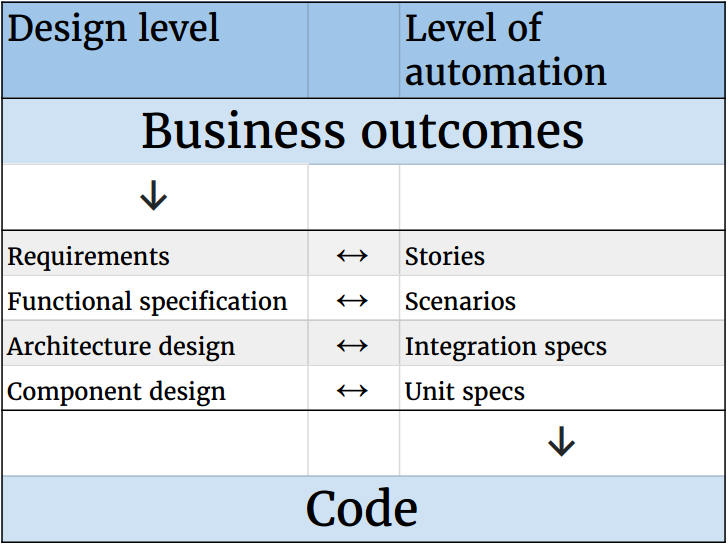
\includegraphics[width=10.0cm]{images/BDD.png}
        \caption{BDD related to system development}
        \label{fig:BDD}
      \end{center}
    \end{figure}

    \textbf{Value} is the \textbf{driving force} to start the progress with features.
    To be implemented, feature must have business value related to business outcomes~\cite{bdd2006north}.
    From there, through different levels of system, implementation is driven with tests first to specify behavior~\cite{chelimsky2010rspec}.
    This all correlates well with quality measured by the earlier introduced alternative quality model. BDD
    process aims to provide features with value in use and high internal \& external software quality. This happens through
    \textit{collaboration, incremental delivery} and \textit{vast \& repeatable automated test suites}~\cite{chelimsky2010rspec}~\cite{smart2014bdd}.
    The outcome should be quality that delights the end user, thus performing well on the AQM~\cite{denning2016sq}.
    Figure \ref{fig:BDD} visualizes how business outcomes and the value derived from them drive the process from outside-in through
    test automation levels to code.

    To fully understand the different levels of automated specification illustrated in figure \ref{fig:BDD}, the whole
    automation level BDD cycle~\cite{chelimsky2010rspec} needs to be explained:
    \begin{figure}[ht]
      \begin{center}
        \includegraphics[width=12.0cm]{images/bdd-cycle.png}
        \caption{Automated BDD cycle}
        \label{fig:bdd-cycle}
      \end{center}
    \end{figure}\newline
    Figure \ref{fig:bdd-cycle} shows the BDD-cycle that can be automated with BDD tools.
    Steps 1 through 4 relate to acceptance level and steps from 5 to 9 are for implementation level. Step #11 is the refactoring
    of acceptance level code. Implementation level steps can be seen as the earlier introduced \textbf{red-green cycle of TDD}, preferably done
    with behavior driven implementation level testing frameworks~\cite{smart2014bdd}. There exists also the outer red-green cycle, which
    is the outside-in aspect of BDD. The development is started with failing acceptance level, which passes later when the
    BDD cycle has progresses through all levels of behavior definition and its implementing code~\cite{chelimsky2010rspec}. By repeating the steps,
    the end result will be a working feature providing value related to business outcomes~\cite{chelimsky2010rspec}.

    \subsection{Levels of specification}
    The first automation level is \textbf{acceptance level} testing ~\cite{chelimsky2010rspec}~\cite{solis2011study}~\cite{smart2014bdd}~\cite{okolnychyi2016study}.
    This level can be seen as a form of ATDD~\cite{gartner2012atdd}. As earlier explained, BDD also includes the ubiquitous language~\cite{bdd2006north}
    from Domain Driven Design and thus all ATDD does not pass as acceptance level BDD.

    At acceptance level, features will be written down as feature files (exact naming depends on the used framework), where they are
    expressed as user stories ~\cite{chelimsky2010rspec}. Acceptance criteria is presented as executable scenarios~\cite{bdd2006north}, that usually
    follow predetermined ubiquitous language \textbf{Gherkin}~\cite{okolnychyi2016study}. Gherkin will be studied in more detail in the next
    chapter when testing framework Spock is examined. Figure \ref{fig:BDD} shows how these stories and scenarios relate to system design.
    The stakeholder audience for acceptance level BDD include all stakeholders interested in development of the product~\cite{smart2014bdd}.

    Some of the BDD acceptance level tools for JVM include \textit{Cucumber-JVM, Concordion} and \textit{JBehave}~\cite{okolnychyi2016study}. Other
    environments have also BDD tools for this level, for instance \textit{SpecFlow} for .NET and \textit{Behave} for Python~\cite{smart2014bdd}.
    Main characteristic of acceptance level tools is business readable plain text input that is expressed with the earlier mentioned
    user stories and their scenarios~\cite{okolnychyi2016study}.

    The second automated level in BDD is \textbf{implementation level} testing ~\cite{chelimsky2010rspec}~\cite{solis2011study}~\cite{smart2014bdd}~\cite{okolnychyi2016study}.
    Implementation level can be seen as testing, where behavior of objects and components are described with examples~\cite{chelimsky2010rspec}.
    This means the earlier mentioned \textit{unit} and \textit{integration} testing done with a new point of view. BDD is not limited to acceptancel level
    only, as one of the core values in it is:
    \textit{"it's all behavior"}~\cite{chelimsky2010rspec}. Every level can be broken down to examples describing behavior.
    Figure \ref{fig:BDD} illustrates how these implementation level specifications relate to system design. Figure \ref{fig:bdd-cycle}
    shows how the two explained automation levels in BDD work together in a cycle.

    Implementation level BDD can be seen to follow the principles of TDD, like the earlier mentioned red-green cycle driving
    the design~\cite{smart2014bdd}. The tests produced by BDD differ from TDD tests, they are more granular pieces of
    describing examples of used code~\cite{astels2006new}. They help to shift the viewpoint from test centric approach by
    changing the often found 1-1 mappings between test cases and test methods to classes and their methods with more descriptive naming~\cite{astels2006new}.

    The outcome from implementation level BDD specifications is readable, behavior oriented living documentation aimed for developers~\cite{chelimsky2010rspec}~\cite{smart2014bdd}.
    Although implementation level BDD can be done with traditional xUnit tools,
    there exists dedicated BDD tools for writing easily \textbf{more concise} and \textbf{more expressive} low level specifications~\cite{smart2014bdd}.
    These implementation level BDD tools provide the base for research work
    in this thesis, therefore they will be examined in more detail later with reviewing testing frameworks \textit{RSpec, Spock} and
    \textit{Spectrum}.

    \subsection{Benefits and drawbacks}

    \begin{table}[H]
        \begin{center}
            \begin{tabular}{ | p{6.3cm} | p{6.3cm} |}
            \hline
            \textbf{Benefits} & \textbf{Drawbacks} \\ \hline
            Frequent collaboration*~\cite{haugset2012automated} & Demands frequent collaboration*~\cite{haugset2012automated}  \\ \hline
            Less ambiquity, noise and over-specification in requirements*~\cite{haugset2012automated} & Needs active customer*~\cite{haugset2012automated}  \\ \hline
            Faster feedback*~\cite{haugset2012automated} & High upfront cost*~\cite{haugset2012automated}  \\ \hline
            Increased requirement traceability*~\cite{hayes2009towards} & Works bad with constantly changing requirements*~\cite{haugset2012automated}  \\ \hline
            Increased trust*~\cite{haugset2012automated} & Learning curve*~\cite{haugset2012automated} \\ \hline
            Increased test coverage*~\cite{haugset2012automated} & Not for all contextes*~\cite{haugset2012automated}  \\ \hline
            Faster start for new team members*~\cite{haugset2012automated} & Requires high discipline*~\cite{haugset2012automated}  \\ \hline
            Ubiquitous language can help in testing right aspects ~\cite{okolnychyi2016study} &  \\ \hline
            Can reduce futile feature development~\cite{smart2014bdd} &  \\ \hline
            \end{tabular}
            \caption {Acceptance Level BDD Benefits \& Drawbacks} \label{tab:bdd-acc-title}
            \caption* {* = No actual source, based on implications}
        \end{center}
    \end{table}
    \textbf{Benefits} (and drawbacks) of \textbf{acceptance level BDD} are almost fully the same as in ATDD. This is the result of
    acceptance level BDD being a form of ATDD~\cite{gartner2012atdd}. Compared to ATDD, Acceptance level BDD introduces the ubiquitous language
    and it can have the effect of changing all stakeholders to think about testing to describe
    behavior instead of internal structures of the system~\cite{okolnychyi2016study}. The emphasis on providing value with
    features can also reduce production of features that are not used~\cite{smart2014bdd}.
    \textbf{Drawbacks} of acceptance level BDD are identical to the earlier mentioned ones of ATDD.

    \begin{table}[H]
        \begin{center}
            \begin{tabular}{ | p{6.3cm} | p{6.3cm} |}
            \hline
            \textbf{Benefits} & \textbf{Drawbacks} \\ \hline
            Increased external quality*~\cite{kollanus2010test}~\cite{bissi2016effects} & Increased\newline development time*~\cite{kollanus2010test}~\cite{bissi2016effects}~\cite{williams2009effectiveness} \\ \hline
            Increased internal quality*~\cite{bissi2016effects} & Requires high discipline~\cite{smart2014bdd} \\ \hline
            Helps to test right aspects of component~\cite{chelimsky2010rspec}~\cite{astels2006new}~\cite{amodeo2015learning} & \\ \hline
            More granular test cases~\cite{chelimsky2010rspec}~\cite{astels2006new} & \\ \hline
            Can help in maintenance~\cite{smart2014bdd} & \\ \hline
            \end{tabular}
            \caption {Implementation Level BDD Benefits \& Drawbacks} \label{tab:bdd-imp-title}
            \caption*{* = No actual source, based on implications}
        \end{center}
    \end{table}
    \textbf{Benefits} of \textbf{implementation level BDD} share the same characteristics of TDD. Although there exists no research
    on how the external and internal quality of software changes with BDD, it should share the same traits as described
    earlier with benefits of TDD. This is a result of implementation level BDD being an evolution of TDD~\cite{astels2006new}.
    As mentioned before, compared to TDD, BDD should help to focus on verifying the right aspects regarding the component.
    This means verifying the behavior of the component instead its structure~\cite{chelimsky2010rspec}~\cite{astels2006new}~\cite{amodeo2015learning}.

    Implementation level BDD aims to produce more granular and descriptive test methods and test cases than TDD~\cite{chelimsky2010rspec}~\cite{astels2006new}.
    These test cases are also describing the behavior of production code by examples~\cite{chelimsky2010rspec}.
    This can help the system maintenance, providing up-to-date documentation for future developers or even the original developer
    later on in the future~\cite{smart2014bdd}.

    \textbf{Drawbacks} of implementation level BDD are not clear, as empirical research on the topic is nonexistent.
    Because of the close relation to TDD, practicing it should introduce a growth in development time~\cite{kollanus2010test}~\cite{bissi2016effects}~\cite{williams2009effectiveness}.
    BDD as whole needs discipline~\cite{smart2014bdd}, therefore it might not be a good fit for all projects and their stakeholders.
    It was also found that BDD is most beneficial when it is used as a holistic approach~\cite{solis2011study}.
    This means including both levels of specification and accommodating working practices to fully support it}.

    As the research on this implementation level of BDD is very limited, this thesis focuses on tools used in it. The main topic of interest is how well
    they could replace traditional xUnit testing family even without tests first principle. Before inspecting these JVM testing
    frameworks in detail, related research about low level testing practices are reviewed.

\section{Related research} % 2p
\label{section:research}
    Although BDD and BDD testing frameworks have been around over a decade, empirical research made on the topic is limited.
    BDD testing frameworks are in heavy use in certain programming languages and frameworks, such as \textit{RSpec} in Ruby on Rails testing~\cite{lerner2009forge},
    \textit{Jasmine} in JavaScript testing~\cite{amodeo2015learning} and \textit{Spock}~\cite{spock} in Groovy testing.
    There exists no exact research on how popular practicing BDD is on the mentioned environments,
    but the reality probably is that these BDD implementation level frameworks are used largely only for testing purposes, not practicing BDD.
    The scope of this thesis is to study the changes in low level testing from introducing BDD implementation level testing
    frameworks without the practice of BDD.
    Therefore, the previous findings in studies done on low level testing are the most important ones regarding this thesis.

    \textbf{Daka and Fraser}~\cite{daka2014survey} studied practitioners of unit testing for used practices and problems in unit testing with a survey.
    They found out that developers are mainly trying to find realistic scenarios on what to test.
    They made important findings of developer perception towards unit testing, such as:
    \begin{itemize}
    \item Developers finding \textit{isolating} of unit under test hard
    \item \textit{Understanding} code is bigger problem than understanding test code
    \item Only half of the survey respondents enjoy writing unit tests
    \item \textit{Maintaining} unit tests was found harder than writing them
    \end{itemize}
    They state that good automated unit tests could help understanding the production code.
    The finding of low enjoyment of practicing unit testing in developers can be seen as troublesome
    and Daka and Fraser notice that there exists a need for tools that rise developer enjoyment in unit testing.
    They also note that there is potential for unit testing research to help developers produce better tests for easier debugging and fixing
    of found defects. It was also discovered that there exists a need for easier maintaining of unit tests.

    \textbf{Li et al}.~\cite{li2016automatically} studied unit testing practices with a developer survey. They specialized in studying
    the documentation of unit testing practices. One general major problem they found out was that 60.38\% of practitioners found understanding of
    unit tests ranging from moderately difficult to very hard. Relevant findings with unit testing documention practices
    were:

    \begin{itemize}
    \item Developers find updated documentation and comments in test cases useful
    \item Writing comments to unit tests is rarely or never done
    \item Developers feel that tests should be self-documenting without comments
    \end{itemize}

    Li et al. state that for effecting maintaining of test cases, it is important for developers to understand the impact and
    functionality of the test case. They also observed that 89.15\% percent of developers agree or strongly agree that maintaining
    of test cases impacts the quality of software system. They conclude that tools for supporting maintaining of unit tests could
    benefit unit test practitioners.

    \textbf{Runeson} ~\cite{runeson2006survey} studied unit testing practices in companies to define unit testing and to evaluate it.
    He states that companies with unclear definition for unit testing face the risk to do bad or inconsistent
    testing. Runeson also found out that unit testing strategies are usually emerging from developers own ambitions, instead of
    management policies.
    Related to problems in unit tests, it was found out that maintaining of unit tests takes much effort. Other
    major problem was developer motivation, which seemed low when working with unit tests.

    Runeson also surveyed developers about documenting practices in unit testing. He found out that unit tests
    are documented preferably in test code rather than in text. He states that motivation to do unit testing in agile projects
    could include test suites functioning as specification.

    \textbf{Williams et al.}~\cite{williams2009effectiveness} studied effectiviness of unit test automation at Microsoft. They also
    surveyed developers about perception towards unit testing.  Around 90\% of developers agree or strongly agree that unit
    tests are useful for regression testing. Around same percentage of developers see unit tests helpful in aiding them to
    produce higher quality code. 60-70\% of developers find unit tests helpful in understanding other peoples code and
    unit tests also helped them to debug found problems.

    \textbf{Berner et al.}~\cite{berner2005observations} report observations from their own and team members experiences of
    automated testing in general. In their experience, test cases at all levels get corrupted easily if they are not
    run frequently. They become inconsistent and difficult to understand. Neglecting test case maintenance effort can result
    in test cases that lose their information value running capability. The cost to restore this type of test cases is very high.
    Berner et al. state that inappropriate testware architecture can cause the observed problems.

    In master's thesis by \textbf{Laplante}~\cite{laplante2009behavior} where she studied differences of TDD and BDD taken into use,
    she found out through a survey that practitioners perceive BDD
    specifications to produce more readable tests than TDD counterparts practiced with \textbf{xUnit family testing frameworks}. Laplante
    also states as interesting future work studying the use of dynamic languages, such as JRuby, for Java testing on the JVM-platform.

    \textbf{In conclusion}, unit testing was found to have many problematic areas from developers perspective.
    These include aspects such as \textit{readability,
    maintainability} and \textit{enjoyment in practicing unit tests}. Many unit testing practitioners also feel the need for
    test code to be \textit{self-documenting}. Implementation level BDD testing tools are advertised to
    help in creating living documentation for the code and also in providing features to help maintaining the test cases~\cite{smart2014bdd}.
    Main topic of interest in later chapters of this thesis is in studying implementation level BDD testing frameworks and
    if they can help with the unit test practitioner problems illustrated in this section.

    Next chapter starts with first examining xUnit testing family tools. These tools are the traditional testing tools in use for the
    related research explained in this section. After that, implementation level BDD testing frameworks are demonstrated in detail
    with examples to see how they differ from the xUnit family.




